\title{Eine mathematisch fundierte Einführung in die Computergrafik}
\author{Johannes Riesterer}
\date{\today}
\maketitle\thispagestyle{empty}
 \begin{figure}[H]
    \centering
    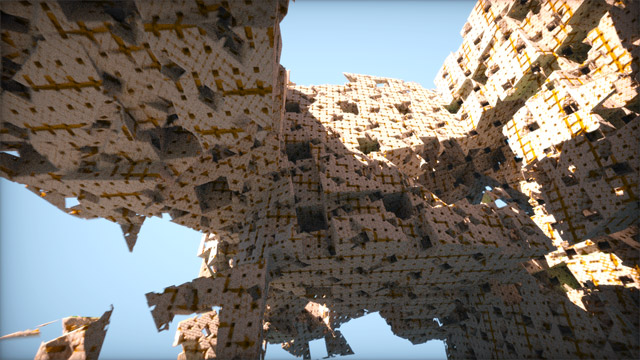
\includegraphics[width=1.0\textwidth]{images/cover.jpg}
    \label{fig:diffus}
\end{figure}
\newpage 
\begin{center}
\large
 \copyright Johannes Riesterer \\
Vervielfältigung nur mit ausdrücklicher Erlaubnis des Autors
\end{center}
\thispagestyle{empty}
\newpage

\section*{Vorwort}
\mbox{}\thispagestyle{empty}

Dieses Skript entstand aus einer Reihe von Vorlesung über Computergrafik, die ich sowohl an der dualen Hochschule in Stuttgart als auch an der Hochschule für 
Kunst Design und populäre Musik Freiburg gehalten habe. Für die Mitarbeit an diesem Skript möchte ich Alexander Berg  danken.



\newpage
